% answers.tex —— 1977 年·广西卷（理科） · 参考答案与详细解析片段
% 由 tools/generate_projects.py 依来源总账自 1977/1977_数学真题_广西理_试题.md + 1977/1977_数学真题_广西理_解析正文.md + 1977/1977_数学真题_广西理_答案要点.md 生成，勿手改（改源 MD 后重跑）


\begin{gktip}
固定源是题面与解答连排的《试题解》扫描材料，题面后紧跟源解答。下文逐题独立推导，并对照源解答复算关键结论。源卷有两处更正预告于此：第 4 题源解答的近似值 $12\sqrt6\approx29.3$ 与四舍五入口径不符（应为 $29.4$）；参考题 1 源解答把原方程组分解为两个子方程组时有两处方程误印（详见该题源注）。
\end{gktip}

\begin{answer}
\gksolhead{1}{}

\textbf{题目}（每小题 5 分，本题 25 分）：

\begin{gktip}
\textbf{题号说明}：源卷第一大题下的五道小题印作「1．—5．」，本库规范要求小问连续编号，故重排为（1）—（5），未增删任何题干内容。
\end{gktip}

（1） $x$ 为何值时，$\dfrac{|x|}{x}$ 的值是？是 $-1$？没有意义？

\begin{gktip}
\textbf{源注}：原卷印作「的值是？」，第一个问句疑漏排数值「1」（源解答应为「的值是 1？」）；本文按原卷保留。
\end{gktip}

（2） 不查表求：$\lg 2-2\lg 4+\lg 5+\lg 16$ 的值。

（3） 计算：$\operatorname{ctg}(-60^\circ)\sin 240^\circ-2\cos(-60^\circ)+\operatorname{tg}^2 150^\circ$。

（4） 计算：$\left(-1\dfrac12\right)^2+81^{\frac34}-(-1)^0\div 0.2+(-2)^{-3}$。

\begin{gktip}
\textbf{源注}：原卷 $(-1)$ 的指数印作小圆圈「°」，源解答按零次幂处理；本文转录为 $(-1)^0$。
\end{gktip}

（5） 求 $A(7,5)$ 和 $B(1,-3)$ 两点间的距离。

\Needspace{4\baselineskip}
\textbf{解析}

\gksubpart{（1）}

\Needspace{5\baselineskip}
$x>0$ 时 $|x|=x$，故

\nopagebreak[4]
\[
\frac{|x|}{x}=1;
\]

\Needspace{5\baselineskip}
$x<0$ 时 $|x|=-x$，故

\nopagebreak[4]
\[
\frac{|x|}{x}=-1;
\]

$x=0$ 时分母为零，$\dfrac{|x|}{x}$ 没有意义。

\gksubpart{（2）}

\Needspace{5\baselineskip}
由 $2\lg4=4\lg2$、$\lg16=4\lg2$，原式

\nopagebreak[4]
\[
\lg2-4\lg2+\lg5+4\lg2=\lg2+\lg5=\lg10=1.
\]

\gksubpart{（3）}

\Needspace{5\baselineskip}
逐项用诱导公式化简：

\nopagebreak[4]
\[
\operatorname{ctg}(-60^\circ)=-\operatorname{ctg}60^\circ=-\frac{\sqrt3}{3},
\]

\nopagebreak[4]
\[
\sin240^\circ=\sin(180^\circ+60^\circ)=-\sin60^\circ=-\frac{\sqrt3}{2},
\]

\nopagebreak[4]
\[
-2\cos(-60^\circ)=-2\cos60^\circ=-1,
\]

\nopagebreak[4]
\[
\operatorname{tg}^2150^\circ=\operatorname{tg}^2(180^\circ-30^\circ)=(-\operatorname{tg}30^\circ)^2=\frac13.
\]

\Needspace{5\baselineskip}
所以

\nopagebreak[4]
\[
\text{\text{原式}}=\frac12-1+\frac13=-\frac16.
\]

\gksubpart{（4）}

\nopagebreak[4]
\[
\left(-1\frac12\right)^2=\frac94,
\qquad
81^{\frac34}=(3^4)^{\frac34}=3^3=27,
\]

\nopagebreak[4]
\[
(-1)^0\div0.2=1\div\frac15=5,
\qquad
(-2)^{-3}=-\frac18.
\]

\Needspace{5\baselineskip}
所以

\nopagebreak[4]
\[
\text{\text{原式}}=\frac94+27-5-\frac18
=\frac{18-1}{8}+22
=24\frac18.
\]

\gksubpart{（5）}

\nopagebreak[4]
\[
|AB|=\sqrt{(7-1)^2+\bigl(5-(-3)\bigr)^2}
=\sqrt{36+64}=10.
\]

\gkanswer{答案（1）：$x>0$ 时 $\dfrac{|x|}{x}=1$；$x<0$ 时 $\dfrac{|x|}{x}=-1$；$x=0$ 时没有意义。}

\gkanswer{答案（2）：$1$。}

\gkanswer{答案（3）：$-\dfrac16$。}

\gkanswer{答案（4）：$24\dfrac18$。}

\gkanswer{答案（5）：$10$。}

\end{answer}
\begin{answer}
\gksolhead{2}{}

\textbf{题目}（20 分）：

红旗机械厂生产 360 台车床，原计划若干天完成，在党的十一大精神舞午下，实际每天比原计划多生产 12 台，结果提前 8 天完成任务。问实际每天生产多少台车床？

\begin{gktip}
\textbf{源注}：原卷印作「精神舞午下」，当为「精神鼓舞下」之误排；本文按原卷保留。
\end{gktip}

\Needspace{4\baselineskip}
\textbf{解析}

\Needspace{5\baselineskip}
设实际每天生产 $x$ 台，则原计划每天生产 $(x-12)$ 台。按原计划完成 360 台需 $\dfrac{360}{x-12}$ 天，实际用了 $\dfrac{360}{x}$ 天，依题意

\nopagebreak[4]
\[
\frac{360}{x-12}-\frac{360}{x}=8.
\]

\Needspace{5\baselineskip}
去分母：

\nopagebreak[4]
\[
360x-360(x-12)=8x(x-12),
\]

\nopagebreak[4]
\[
8x^2-96x-4320=0
\quad\Longrightarrow\quad
x^2-12x-540=0,
\]

\nopagebreak[4]
\[
(x-30)(x+18)=0,
\qquad
x=30\ \text{\text{或}}\ x=-18.
\]

$x=-18$ 为负数，不合题意舍去；把 $x=30$ 代入原方程分母 $x(x-12)=540\ne0$，是原方程的根。复核：原计划每天 18 台需 20 天，实际每天 30 台只需 12 天，恰提前 8 天，与题设相符。

\gkanswer{答案：实际每天生产 $30$ 台。}

\end{answer}
\begin{answer}
\gksolhead{3}{}

\textbf{题目}（17 分）：

在四边形 $ABCD$ 中，$E\text{、}F$ 分别是对角线 $AC\text{、}BD$ 的中点，$M\text{、}N$ 分别是 $AB\text{、}CD$ 的中点，求证 $EF$ 与 $MN$ 互相平分。
\nopagebreak[4]
\begin{center}% 1977 年广西卷（理科）第 3 题：四边形 ABCD，E、F 为对角线 AC、BD 的中点，M、N 为 AB、CD 的中点，
% 虚线四边形 EMFN 为平行四边形，MN、EF 是其对角线（按源卷第 2 页布局）
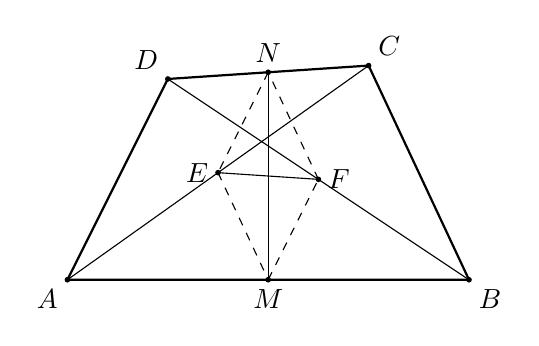
\begin{tikzpicture}[scale=0.85]
  \coordinate (A) at (0,0);
  \coordinate (B) at (6,0);
  \coordinate (D) at (1.5,3);
  \coordinate (C) at (4.5,3.2);
  \coordinate (M) at (3,0);
  \coordinate (N) at (3,3.1);
  \coordinate (E) at (2.25,1.6);
  \coordinate (F) at (3.75,1.5);
  \draw[thick] (A)--(B)--(C)--(D)--cycle;
  \draw[thin] (A)--(C);
  \draw[thin] (B)--(D);
  \draw (E)--(F);
  \draw (M)--(N);
  \draw[dashed] (E)--(M) (M)--(F) (F)--(N) (N)--(E);
  \fill (A) circle (1.2pt) node[below left] {$A$};
  \fill (B) circle (1.2pt) node[below right] {$B$};
  \fill (C) circle (1.2pt) node[above right] {$C$};
  \fill (D) circle (1.2pt) node[above left] {$D$};
  \fill (M) circle (1.2pt) node[below] {$M$};
  \fill (N) circle (1.2pt) node[above] {$N$};
  \fill (E) circle (1.2pt) node[left] {$E$};
  \fill (F) circle (1.2pt) node[right] {$F$};
\end{tikzpicture}
\end{center}
\nopagebreak[4]
\Needspace{4\baselineskip}
\textbf{解析}
\nopagebreak[4]
\begin{center}% 1977 年广西卷（理科）第 3 题：四边形 ABCD，E、F 为对角线 AC、BD 的中点，M、N 为 AB、CD 的中点，
% 虚线四边形 EMFN 为平行四边形，MN、EF 是其对角线（按源卷第 2 页布局）
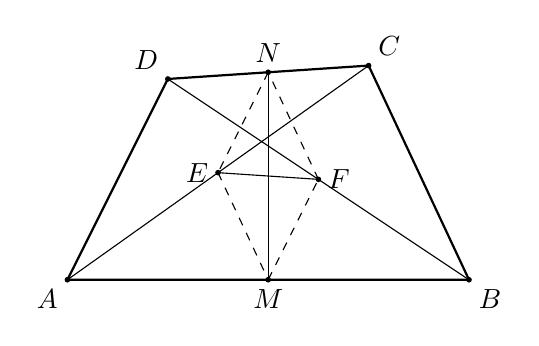
\begin{tikzpicture}[scale=0.85]
  \coordinate (A) at (0,0);
  \coordinate (B) at (6,0);
  \coordinate (D) at (1.5,3);
  \coordinate (C) at (4.5,3.2);
  \coordinate (M) at (3,0);
  \coordinate (N) at (3,3.1);
  \coordinate (E) at (2.25,1.6);
  \coordinate (F) at (3.75,1.5);
  \draw[thick] (A)--(B)--(C)--(D)--cycle;
  \draw[thin] (A)--(C);
  \draw[thin] (B)--(D);
  \draw (E)--(F);
  \draw (M)--(N);
  \draw[dashed] (E)--(M) (M)--(F) (F)--(N) (N)--(E);
  \fill (A) circle (1.2pt) node[below left] {$A$};
  \fill (B) circle (1.2pt) node[below right] {$B$};
  \fill (C) circle (1.2pt) node[above right] {$C$};
  \fill (D) circle (1.2pt) node[above left] {$D$};
  \fill (M) circle (1.2pt) node[below] {$M$};
  \fill (N) circle (1.2pt) node[above] {$N$};
  \fill (E) circle (1.2pt) node[left] {$E$};
  \fill (F) circle (1.2pt) node[right] {$F$};
\end{tikzpicture}
\end{center}
\nopagebreak[4]
\Needspace{5\baselineskip}
在 $\triangle ACD$ 中，$E\text{、}N$ 分别是 $AC\text{、}CD$ 的中点，由三角形中位线定理

\nopagebreak[4]
\[
EN\ \underline{\parallel}\ \frac12AD
\]

\Needspace{5\baselineskip}
（即 $EN\parallel AD$ 且 $EN=\dfrac12AD$）。在 $\triangle ABD$ 中，$M\text{、}F$ 分别是 $AB\text{、}BD$ 的中点，同理

\nopagebreak[4]
\[
MF\ \underline{\parallel}\ \frac12AD.
\]

\Needspace{5\baselineskip}
由平行公理 $MF\parallel EN$ 且 $MF=EN$，所以四边形 $MFNE$ 为平行四边形。$MN$ 与 $EF$ 是它的两条对角线，平行四边形对角线互相平分，故

\nopagebreak[4]
\[
EF\ \text{\text{与}}\ MN\ \text{\text{互相平分}}.
\]

\gkanswer{答案：见解析版}

\end{answer}
\begin{answer}
\gksolhead{4}{}

\textbf{题目}（18 分）：

已知正四棱锥底面边长为 $6$ 厘米，侧棱是高的 $2$ 倍。求这棱锥的体积。（精确到 $0.1$ 立方厘米）
\nopagebreak[4]
\begin{center}% 1977 年广西卷（理科）第 4 题：正四棱锥 V-ABCD，O 为底面正方形中心（高的垂足），
% 实线：可见侧棱 VA、VB、VC 与底边 AB、BC；虚线：侧棱 VD、底边 AD、DC、高 VO、底面对角线半段 AO、DO（按源卷第 3 页布局）
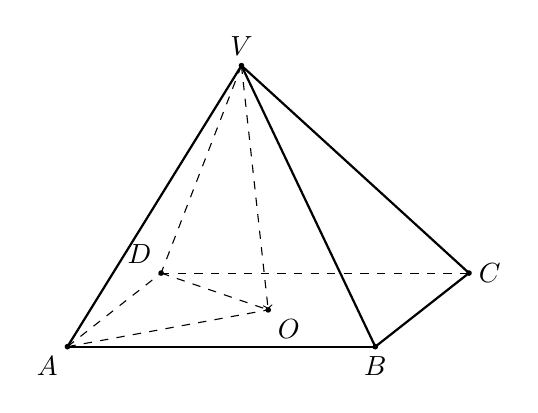
\begin{tikzpicture}[scale=0.85]
  \coordinate (A) at (0,0);
  \coordinate (B) at (4.6,0);
  \coordinate (C) at (6,1.1);
  \coordinate (D) at (1.4,1.1);
  \coordinate (O) at (3,0.55);
  \coordinate (V) at (2.6,4.2);
  \draw[thick] (V)--(A);
  \draw[thick] (V)--(B);
  \draw[thick] (V)--(C);
  \draw[thick] (A)--(B);
  \draw[thick] (B)--(C);
  \draw[dashed] (V)--(D);
  \draw[dashed] (A)--(D);
  \draw[dashed] (D)--(C);
  \draw[dashed,->] (V)--(O);
  \draw[dashed] (A)--(O);
  \draw[dashed] (D)--(O);
  \fill (A) circle (1.2pt) node[below left] {$A$};
  \fill (B) circle (1.2pt) node[below] {$B$};
  \fill (C) circle (1.2pt) node[right] {$C$};
  \fill (D) circle (1.2pt) node[above left] {$D$};
  \fill (O) circle (1.2pt) node[below right] {$O$};
  \fill (V) circle (1.2pt) node[above] {$V$};
\end{tikzpicture}
\end{center}
\nopagebreak[4]
\Needspace{4\baselineskip}
\textbf{解析}
\nopagebreak[4]
\begin{center}% 1977 年广西卷（理科）第 4 题：正四棱锥 V-ABCD，O 为底面正方形中心（高的垂足），
% 实线：可见侧棱 VA、VB、VC 与底边 AB、BC；虚线：侧棱 VD、底边 AD、DC、高 VO、底面对角线半段 AO、DO（按源卷第 3 页布局）
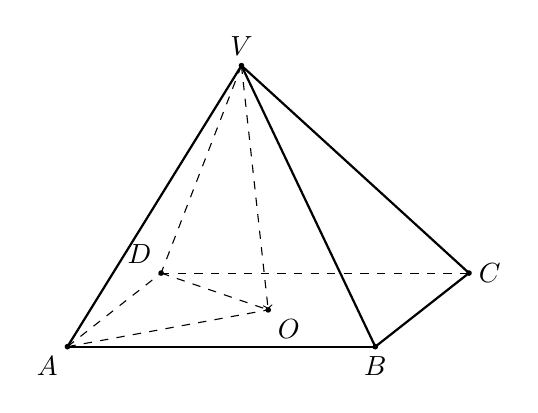
\begin{tikzpicture}[scale=0.85]
  \coordinate (A) at (0,0);
  \coordinate (B) at (4.6,0);
  \coordinate (C) at (6,1.1);
  \coordinate (D) at (1.4,1.1);
  \coordinate (O) at (3,0.55);
  \coordinate (V) at (2.6,4.2);
  \draw[thick] (V)--(A);
  \draw[thick] (V)--(B);
  \draw[thick] (V)--(C);
  \draw[thick] (A)--(B);
  \draw[thick] (B)--(C);
  \draw[dashed] (V)--(D);
  \draw[dashed] (A)--(D);
  \draw[dashed] (D)--(C);
  \draw[dashed,->] (V)--(O);
  \draw[dashed] (A)--(O);
  \draw[dashed] (D)--(O);
  \fill (A) circle (1.2pt) node[below left] {$A$};
  \fill (B) circle (1.2pt) node[below] {$B$};
  \fill (C) circle (1.2pt) node[right] {$C$};
  \fill (D) circle (1.2pt) node[above left] {$D$};
  \fill (O) circle (1.2pt) node[below right] {$O$};
  \fill (V) circle (1.2pt) node[above] {$V$};
\end{tikzpicture}
\end{center}
\nopagebreak[4]
\Needspace{5\baselineskip}
设高为 $VO=h$，侧棱 $VA=2h$。正四棱锥顶点在底面的射影 $O$ 是底面正方形的中心，

\nopagebreak[4]
\[
AO=DO=\frac{\sqrt2}{2}\times6=3\sqrt2.
\]

\Needspace{5\baselineskip}
在 $\mathrm{Rt}\triangle VOA$ 中由勾股定理

\nopagebreak[4]
\[
VA^2=VO^2+AO^2,
\qquad
4h^2=h^2+18,
\qquad
h^2=6,
\qquad
h=\sqrt6.
\]

\Needspace{5\baselineskip}
所以

\nopagebreak[4]
\[
V_{\text{\text{棱锥}}}=\frac13\times6^2\times\sqrt6=12\sqrt6\approx29.4\ \text{（\text{立方厘米}）}.
\]

\begin{gktip}
\textbf{源注}：源解答印作「$12\sqrt6\approx29.3$（厘米³）」。$12\sqrt6=29.39\cdots$，按题设「精确到 $0.1$ 立方厘米」的四舍五入口径应为 $29.4$；源卷的 $29.3$ 系直接截断。本文按四舍五入收录 $29.4$。
\end{gktip}

\gkanswer{答案：$V=12\sqrt6\approx29.4$ 立方厘米。}

\end{answer}
\begin{answer}
\gksolhead{5}{}

\textbf{题目}（20 分）：

把一块钢板冲成上面是半园形、下面是矩形的零件，已知零件的周长是 $P$，怎样才能使冲出的零件面积最大？
\nopagebreak[4]
\begin{center}% 1977 年广西卷（理科）第 5 题：上部半园、下部矩形的零件，矩形宽 x 标于底边下方（按源卷第 3 页布局）
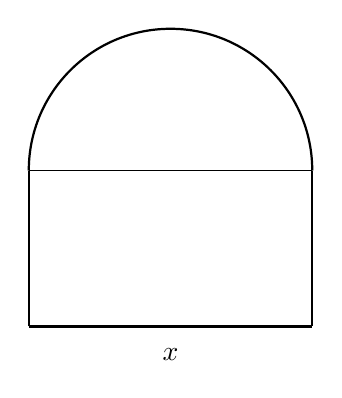
\begin{tikzpicture}[scale=0.9]
  \draw[thick] (0,0)--(4,0);
  \draw[thick] (0,0)--(0,2.2);
  \draw[thick] (4,0)--(4,2.2);
  \draw[thin] (0,2.2)--(4,2.2);
  \draw[thick] (0,2.2) arc(180:0:2);
  \node at (2,-0.4) {$x$};
\end{tikzpicture}
\end{center}
\nopagebreak[4]
\begin{gktip}
\textbf{参考题说明}：源卷第五题后印有「〔选作题〕考生可根据自己能力选作，作为参考成绩，不列入总分」，其下两题沿用大题号「一、二」编号。本库改题为参考题 1、2，不计入正式题量。
\end{gktip}

\Needspace{5\baselineskip}
\textbf{参考题 1．} 解方程组

\nopagebreak[4]
\[
\begin{cases}
\sqrt[3]{(x+y)^2}+2\sqrt[3]{(x-y)^2}=3\sqrt[3]{x^2-y^2},\\
3x-2y=13.
\end{cases}
\]

\textbf{参考题 2．} 线段 $AB$ 之三等分点依次为 $C\text{、}D$，以 $CD$ 为直径画园，在园周上任取一点 $P$。求证 $\operatorname{tg}\angle APC\cdot\operatorname{tg}\angle BPD=\dfrac14$。
\nopagebreak[4]
\begin{center}% 1977 年广西卷（理科）参考题 2：线段 AB 上 C、D 为三等分点，以 CD 为直径作园，P 为园周上一点，
% PE 垂直 AB 于 E，θ 为 PC 与 CD 的夹角（按源卷第 5 页布局）
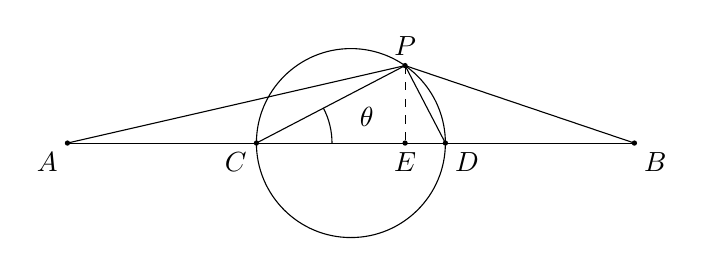
\begin{tikzpicture}[scale=0.8]
  \coordinate (A) at (0,0);
  \coordinate (C) at (3,0);
  \coordinate (D) at (6,0);
  \coordinate (B) at (9,0);
  \coordinate (P) at (5.36,1.23);
  \coordinate (E) at (5.36,0);
  \draw (A)--(B);
  \draw (4.5,0) circle (1.5);
  \draw (A)--(P);
  \draw (B)--(P);
  \draw (P)--(C);
  \draw (P)--(D);
  \draw[dashed] (P)--(E);
  \draw (4.2,0) arc(0:27.5:1.2);
  \node at (4.75,0.42) {$\theta$};
  \fill (A) circle (1.2pt) node[below left] {$A$};
  \fill (B) circle (1.2pt) node[below right] {$B$};
  \fill (C) circle (1.2pt) node[below left] {$C$};
  \fill (D) circle (1.2pt) node[below right] {$D$};
  \fill (E) circle (1.2pt) node[below] {$E$};
  \fill (P) circle (1.2pt) node[above] {$P$};
\end{tikzpicture}
\end{center}
\nopagebreak[4]
\Needspace{4\baselineskip}
\textbf{解析}
\nopagebreak[4]
\begin{center}% 1977 年广西卷（理科）第 5 题：上部半园、下部矩形的零件，矩形宽 x 标于底边下方（按源卷第 3 页布局）
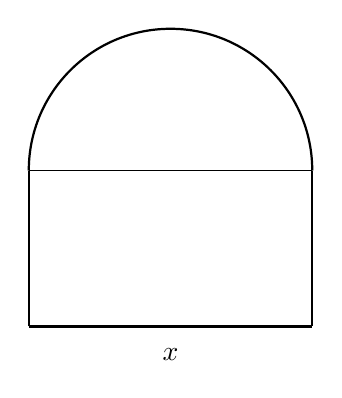
\begin{tikzpicture}[scale=0.9]
  \draw[thick] (0,0)--(4,0);
  \draw[thick] (0,0)--(0,2.2);
  \draw[thick] (4,0)--(4,2.2);
  \draw[thin] (0,2.2)--(4,2.2);
  \draw[thick] (0,2.2) arc(180:0:2);
  \node at (2,-0.4) {$x$};
\end{tikzpicture}
\end{center}
\nopagebreak[4]
\Needspace{5\baselineskip}
设矩形的宽为 $x$（即半园的直径），高为 $h$，零件面积为 $S$。半园的弧长为 $\dfrac{\pi x}{2}$，零件周长

\nopagebreak[4]
\[
P=\frac{\pi x}{2}+2h+x
\quad\Longrightarrow\quad
h=\frac12\left(P-\frac{\pi x}{2}-x\right)
=\frac{2P-(\pi+2)x}{4}.
\]

\Needspace{5\baselineskip}
零件面积 = 半园面积 + 矩形面积：

\nopagebreak[4]
\[
S=\frac{\pi}{2}\left(\frac{x}{2}\right)^2+xh
=\frac{\pi x^2}{8}+\frac{2Px-(\pi+2)x^2}{4}
=-\frac{\pi+4}{8}x^2+\frac{P}{2}x.
\]

\Needspace{5\baselineskip}
这是 $S$ 关于 $x$ 的二次函数，开口向下（$a=-\dfrac{\pi+4}<0$），在

\nopagebreak[4]
\[
x=-\frac{b}{2a}=\frac{P/2}{2\times\dfrac{\pi+4}{8}}=\frac{2P}{\pi+4}
\]

\Needspace{5\baselineskip}
处取最大值。此时

\nopagebreak[4]
\[
h=\frac{2P-(\pi+2)\cdot\dfrac{2P}{\pi+4}}{4}
=\frac{P}{\pi+4},
\]

\Needspace{5\baselineskip}
宽与高之比

\nopagebreak[4]
\[
x:h=\frac{2P}{\pi+4}:\frac{P}{\pi+4}=2:1.
\]

即当矩形的宽为 $\dfrac{2P}{\pi+4}$、高为 $\dfrac{P}{\pi+4}$（宽：高 $=2:1$）时，冲出的零件面积最大。

\textbf{参考题 1}

\begin{gktip}
\textbf{题号说明}：以下两题为源卷「〔选作题〕」（沿用大题号「一、二」），本库改题为参考题 1、2，不计入正式题量，本卷正式题止于第 5 题。
\end{gktip}

\Needspace{5\baselineskip}
设 $t=\sqrt[3]{x+y}$，$s=\sqrt[3]{x-y}$（$t\text{、}s$ 均为实数），则

\nopagebreak[4]
\[
\sqrt[3]{(x+y)^2}=t^2,
\qquad
\sqrt[3]{(x-y)^2}=s^2,
\qquad
\sqrt[3]{x^2-y^2}=\sqrt[3]{(x+y)(x-y)}=ts.
\]

\Needspace{5\baselineskip}
方程 $\sqrt[3]{(x+y)^2}+2\sqrt[3]{(x-y)^2}=3\sqrt[3]{x^2-y^2}$ 化为

\nopagebreak[4]
\[
t^2+2s^2=3ts
\quad\Longrightarrow\quad
(t-s)(t-2s)=0,
\]

所以 $t=s$ 或 $t=2s$。

\textbf{（i）} $t=s$ 时，$x+y=x-y$，得 $y=0$；代入 $3x-2y=13$ 得 $x=\dfrac{13}{3}$。

\Needspace{5\baselineskip}
\textbf{（ii）} $t=2s$ 时，两边立方，$x+y=8(x-y)$，即 $7x-9y=0$；与 $3x-2y=13$ 联立，由 $x=\dfrac97 y$ 得

\nopagebreak[4]
\[
\frac{27}{7}y-2y=13
\quad\Longrightarrow\quad
\frac{13}{7}y=13
\quad\Longrightarrow\quad
y=7,
\qquad
x=9.
\]

\Needspace{5\baselineskip}
两组解代入原方程组均满足（$(x,y)=\left(\dfrac{13}{3},0\right)$ 时第一式两边同为 $3\sqrt[3]{\left(\dfrac{13}{3}\right)^2}$；$(9,7)$ 时 $\sqrt[3]{16^2}+2\sqrt[3]{2^2}=3\sqrt[3]{32}$ 成立），故原方程组的解为

\nopagebreak[4]
\[
\begin{cases}
x_1=\dfrac{13}{3},\\
y_1=0,
\end{cases}
\qquad
\begin{cases}
x_2=9,\\
y_2=7.
\end{cases}
\]

\begin{gktip}
\textbf{源注}：源解答在分解方程组处有两处排印错误：一处把第二条方程印作「$3x-2x=13$」，另一处印作「$3x-2y=0$」，均应为 $3x-2y=13$；源解答所得两组解与本文一致。
\end{gktip}

\textbf{参考题 2}

\Needspace{4\baselineskip}
\textbf{解析}
\nopagebreak[4]
\begin{center}% 1977 年广西卷（理科）参考题 2：线段 AB 上 C、D 为三等分点，以 CD 为直径作园，P 为园周上一点，
% PE 垂直 AB 于 E，θ 为 PC 与 CD 的夹角（按源卷第 5 页布局）
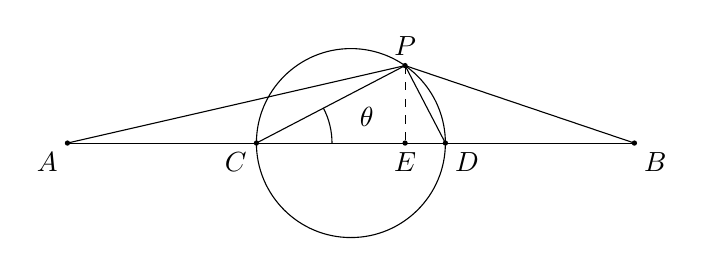
\begin{tikzpicture}[scale=0.8]
  \coordinate (A) at (0,0);
  \coordinate (C) at (3,0);
  \coordinate (D) at (6,0);
  \coordinate (B) at (9,0);
  \coordinate (P) at (5.36,1.23);
  \coordinate (E) at (5.36,0);
  \draw (A)--(B);
  \draw (4.5,0) circle (1.5);
  \draw (A)--(P);
  \draw (B)--(P);
  \draw (P)--(C);
  \draw (P)--(D);
  \draw[dashed] (P)--(E);
  \draw (4.2,0) arc(0:27.5:1.2);
  \node at (4.75,0.42) {$\theta$};
  \fill (A) circle (1.2pt) node[below left] {$A$};
  \fill (B) circle (1.2pt) node[below right] {$B$};
  \fill (C) circle (1.2pt) node[below left] {$C$};
  \fill (D) circle (1.2pt) node[below right] {$D$};
  \fill (E) circle (1.2pt) node[below] {$E$};
  \fill (P) circle (1.2pt) node[above] {$P$};
\end{tikzpicture}
\end{center}
\nopagebreak[4]
\Needspace{5\baselineskip}
设 $AC=CD=DB=a$，记 $\theta=\angle PCD$。因为 $CD$ 是园的直径而 $P$ 在园周上，由直径所对的园周角是直角，$\angle CPD=90^\circ$。在 $\mathrm{Rt}\triangle PCD$ 中

\nopagebreak[4]
\[
PC=a\cos\theta,
\qquad
PD=a\sin\theta.
\]

\Needspace{5\baselineskip}
作 $PE\perp AB$，垂足为 $E$。在 $\mathrm{Rt}\triangle PCE$ 中（斜边为 $PC$）

\nopagebreak[4]
\[
PE=PC\sin\theta=a\sin\theta\cos\theta,
\qquad
CE=PC\cos\theta=a\cos^2\theta.
\]

\Needspace{5\baselineskip}
于是

\nopagebreak[4]
\[
AE=AC+CE=a(1+\cos^2\theta),
\qquad
DE=CD-CE=a(1-\cos^2\theta)=a\sin^2\theta,
\]

\nopagebreak[4]
\[
BE=BD+DE=a(1+\sin^2\theta).
\]

\Needspace{5\baselineskip}
所以

\nopagebreak[4]
\[
\operatorname{tg}A=\frac{PE}{AE}
=\frac{\sin\theta\cos\theta}{1+\cos^2\theta}
=\frac{\operatorname{tg}\theta}{2+\operatorname{tg}^2\theta},
\qquad
\operatorname{tg}B=\frac{PE}{BE}
=\frac{\sin\theta\cos\theta}{1+\sin^2\theta}
=\frac{\operatorname{tg}\theta}{1+2\operatorname{tg}^2\theta}.
\]

\Needspace{5\baselineskip}
在 $\triangle APC$ 中，$\angle ACP=180^\circ-\theta$，故 $\angle APC=180^\circ-A-(180^\circ-\theta)=\theta-A$，从而

\nopagebreak[4]
\[
\operatorname{tg}\angle APC
=\operatorname{tg}(\theta-A)
=\frac{\operatorname{tg}\theta-\operatorname{tg}A}{1+\operatorname{tg}\theta\cdot\operatorname{tg}A}.
\]

\Needspace{5\baselineskip}
记 $t=\operatorname{tg}\theta$，把 $\operatorname{tg}A=\dfrac{t}{2+t^2}$ 代入：

\nopagebreak[4]
\[
\operatorname{tg}\angle APC
=\frac{t-\dfrac{t}{2+t^2}}{1+\dfrac{t^2}{2+t^2}}
=\frac{t(1+t^2)}{2+2t^2}
=\frac{t}{2}.
\]

\Needspace{5\baselineskip}
在 $\triangle PBD$ 中，$\angle PDC=90^\circ-\theta$（$\triangle PCD$ 的内角），而 $D$ 处的外角补角给出 $\angle PDB=180^\circ-(90^\circ-\theta)=90^\circ+\theta$，故

\nopagebreak[4]
\[
\angle BPD=180^\circ-(90^\circ+\theta)-B=90^\circ-\theta-B,
\]

\nopagebreak[4]
\[
\operatorname{tg}\angle BPD
=\operatorname{tg}\bigl(90^\circ-(\theta+B)\bigr)
=\operatorname{ctg}(\theta+B)
=\frac{1-\operatorname{tg}\theta\cdot\operatorname{tg}B}{\operatorname{tg}\theta+\operatorname{tg}B}.
\]

\Needspace{5\baselineskip}
把 $\operatorname{tg}B=\dfrac{t}{1+2t^2}$ 代入：

\nopagebreak[4]
\[
\operatorname{tg}\angle BPD
=\frac{1-\dfrac{t^2}{1+2t^2}}{t+\dfrac{t}{1+2t^2}}
=\frac{1+t^2}{2t(1+t^2)}
=\frac{1}{2t}.
\]

\Needspace{5\baselineskip}
两式相乘，

\nopagebreak[4]
\[
\operatorname{tg}\angle APC\cdot\operatorname{tg}\angle BPD
=\frac{t}{2}\cdot\frac{1}{2t}
=\frac14.
\]

命题得证。

\gkanswer{答案：矩形的宽为 $\dfrac{2P}{\pi+4}$、高为 $\dfrac{P}{\pi+4}$，即宽与高之比为 $2:1$ 时，冲出的零件面积最大。}

\end{answer}